\documentclass[12pt]{report}

%Tous les packets
\usepackage{luatextra}
\usepackage{hyperref}
\usepackage{hhline}
\usepackage{multirow}
\usepackage{listings}
\usepackage{fancyhdr}
\usepackage[french]{babel}
\usepackage{lastpage}
\usepackage{amsmath}
\usepackage{float}
\usepackage[center]{caption}
\usepackage{enumitem}
%Page de garde
\title{Rapport Projet informatique 2020 :\\Site de rencontre}
\author{Florent \textsc{Bednarek} \and Théo \textsc{Julien} \and Julien \textsc{Richard}\and William \textsc{Kaczmarek}}
\date{20  avril au 21 juin 2020}
%Constantes pour tout le document
\usepackage[a4paper, left=1cm, right=1cm, top=2.5cm, bottom=2.5cm]{geometry}
\makeatletter
\let\theauthor\@author
\let\thetitle\@title
\makeatother

%Style du document entier
\pagestyle{fancy}
\renewcommand{\thesection}{\Roman{section}}
\fancyhead[R]{Site de rencontre}
\fancyhead[L]{CPI2 2019-2020}
\renewcommand\footrulewidth{1pt}
\fancyfoot[R]{\thepage /\pageref{LastPage}}
\fancyfoot[C]{}
\fancyfoot[L]{Bednarek, Julien, Kaczmarek, Richard}

\begin{document}
	\maketitle
	\tableofcontents
	\clearpage
\section{Introduction} 
	Pour terminer le module d'informatique cette année nous avons comme à notre habitude un projet de groupe à réaliser. Ce projet en groupe de 3 ou 4 étudiants, se déroule pendant 8 semaines environ. Laissant presque carte blanche à chaque groupe sur un thème sélectionnée. Nous avions à notre disposition 3 thèmes : \\
\begin{itemize}
	\item un site de services (du style AirBnB, Blablacar, etc...)
	\item un site rencontre
	\item un site d'e-commerce (Leboncoin, etc...)\\
\end{itemize}
Voulant avant tout s'amuser le plus possible, nous avons trouvé que le thème "site de rencontre" était le plus intéressant et avec le plus de défi.\\
\\
Nous devions tout d'abord trouver une spécificité à notre site. Nous avons voulu créer un site où l'authenticité était le principal point. Nous voulions à tout pris éviter les profils FAKE(=Faux), qui vendent des service externes et pollue l'application. Nous voulions aussi éviter que les gens mentent sur leur âges, en effet il est fréquent que des enfants ou adolescent s'inscrivent sur des applications en mentant sur leur âges. Ou encore des personnes se rajeunissant. Dans cette optique nous avons voulu réserver notre application aux étudiants, comme cela nous évitions les problèmes cité ci-dessus. En effet, en demandant la carte étudiante à l'inscription nous pouvions vérifier l'authenticité de la personne ainsi que son âge, même si celle-ci ment dessus si elle est étudiant elle sera forcément dans un tranche d'âges des autres utilisateurs. \\
\\ 
\begin{figure}[h!]
	\begin{center}
		
\includegraphics[scale=0.3]{intro.jpg}
	\end{center}
		\caption{Icone de différent site de recontre}
\end{figure}
\clearpage

\section{Notre projet/site}
	Quand on arrive pour la première fois sur notre site, on voit de suite deux boutons un pour la connexion et l'autre pour l'inscription. Nous avons fais le choix de ne pas permettre à un visiteur non inscrit de voir les profils de nos utilisateurs.
	\subsection{Inscription}
	Lorsqu'on clique sur se créer un compte une interface apparait permettant au visiteur de s'enregistrer. Pour cela il faut qu'il fournisse son : Nom, Prénom, Ville, adresse mail et enfin un mot de passe de compte qu'il devra confirmer.\\
	On remarque lorsqu'on commence à rentrer notre ville, au dessus de la zone une ville apparait selon les caractères inscrit. C'est l'API d'adresse du gouvernement français qui détecte la ville, cela nous permet de récupérer la position exact du visiteur afin de savoir à combien de km le séparera des autres profils.\\
On remarque aussi que lorsqu'on commence à taper notre mot de passe une barre de couleur apparait en dessous, cela est la force de notre mot de passe. Une fois toutes les données entrées on clique sur "s'enregistrer". Si tout va bien, une nouvelle interface apparait nous indiquant que notre compte à bien été crée, et nous propose alors d'envoyer notre carte étudiante cette étape permet de vérifier notre compte. Cette carte étudiante ne doit pas dépasser 2 Mo, et peut être au format .png/.jpg/.jpeg.\\
Si l'on upload notre carte la création du compte est terminée , dans le cas où l'on upload pas notre carte nous pouvons quand même nous connecter et dans notre profil on pourra upload notre carte étudiante.
\subsection{Connexion}
	Lorsqu'on clique sur le bouton connexion une interface classique de connexion apparait pour nous connecter. Une fois connecter on se retrouve directement sur l'interface principale.
\begin{figure}[h!]
	\begin{center}
		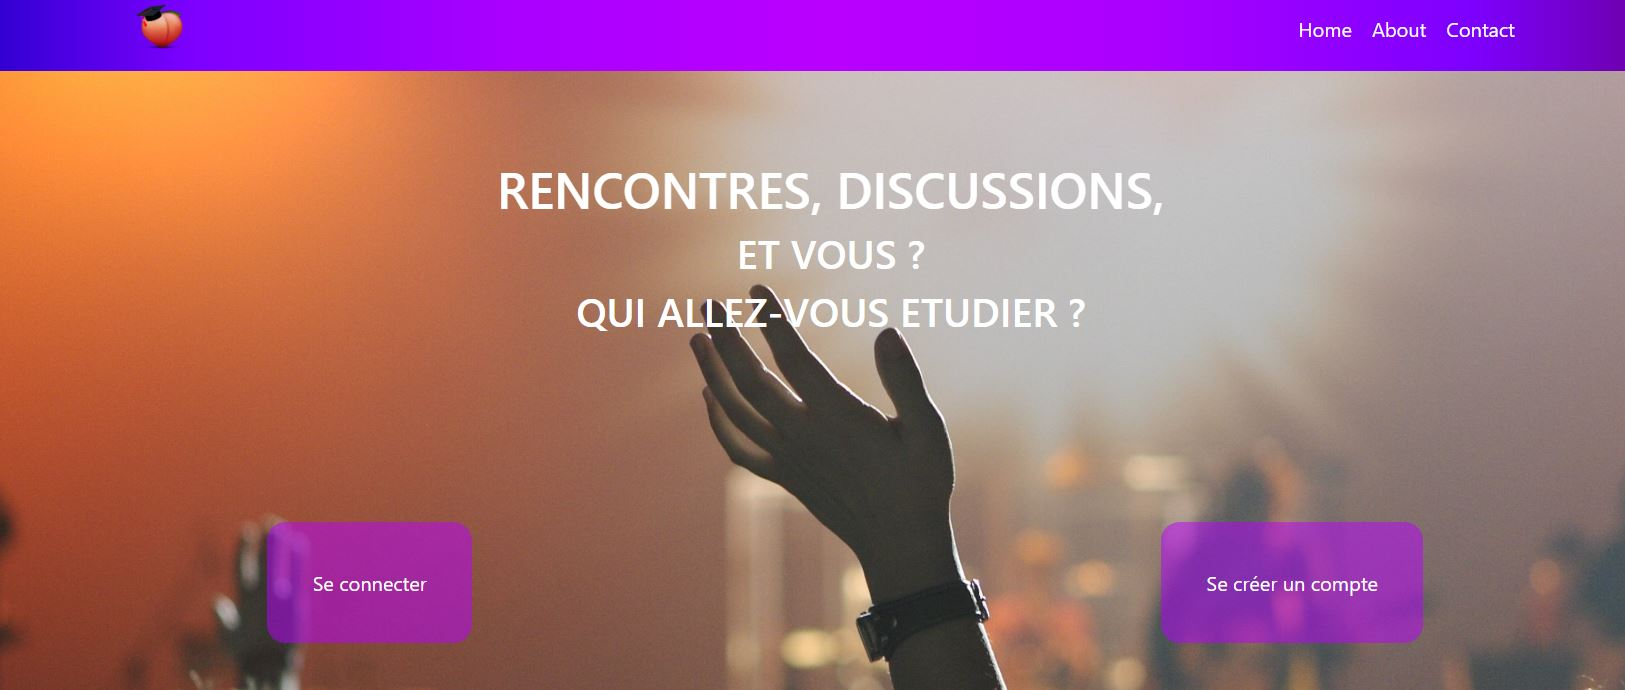
\includegraphics[scale=0.5]{acceuil.jpg}
	\end{center}
		\caption{Capture d'écran de notre site}
\end{figure}
\clearpage
\subsection{Acceuil}
\begin{figure}[h!]
	\begin{center}
		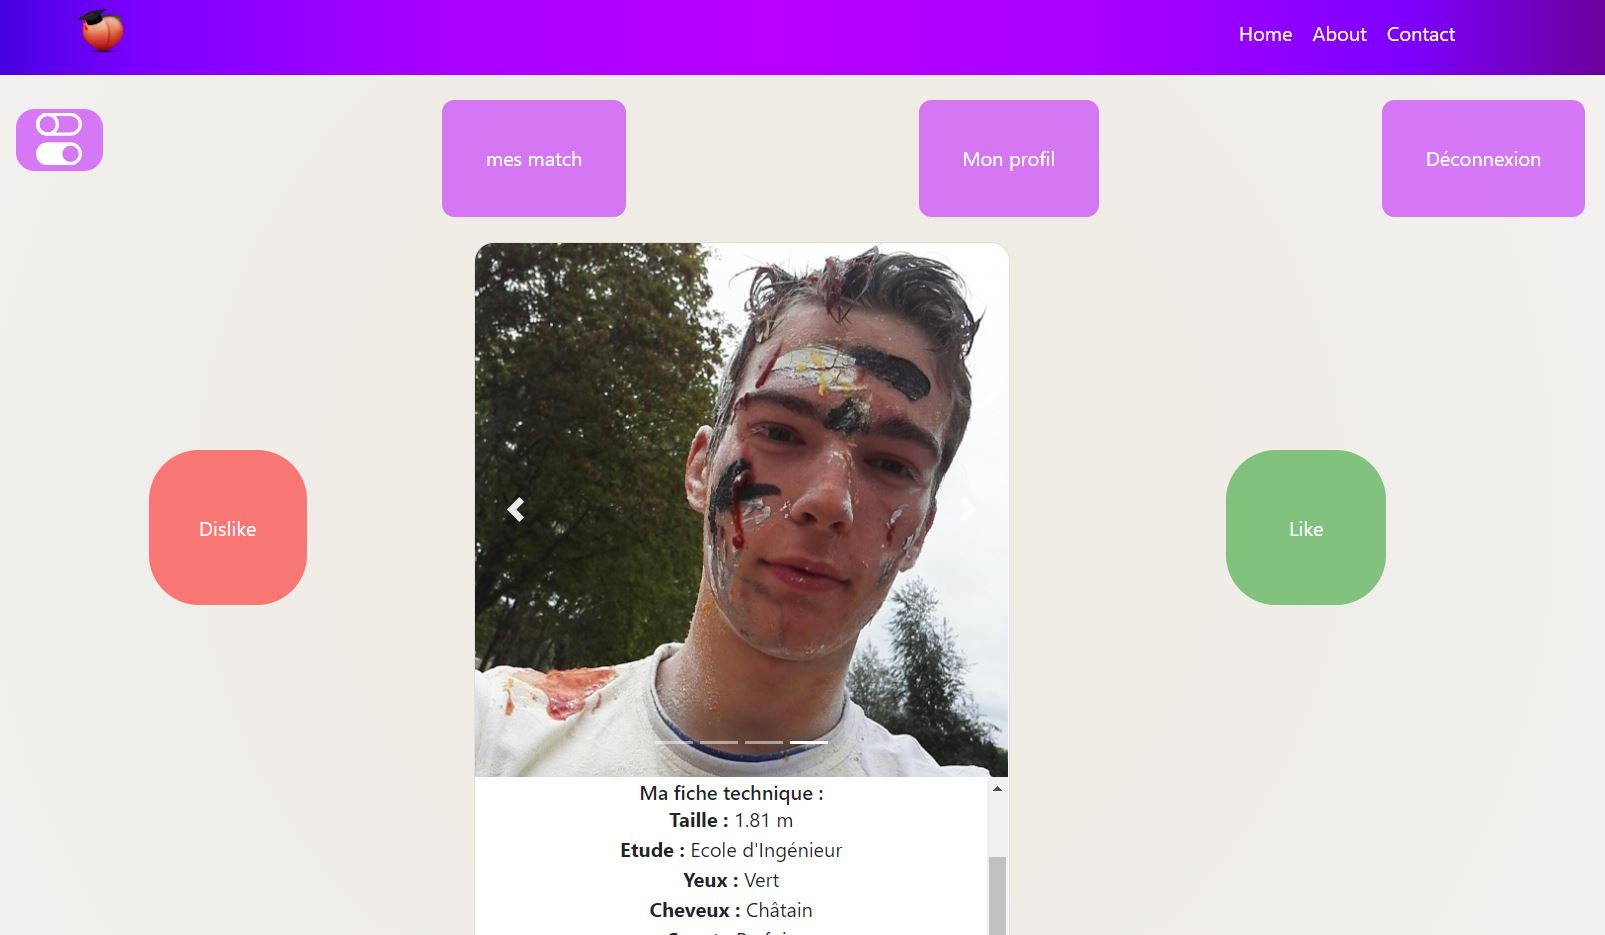
\includegraphics[scale=0.5]{principal.jpg}
	\end{center}
		\caption{Capture d'écran de notre site une fois connecté (sur un profil non administrateur}
\end{figure}
Nous voila enfin sur la page principal on peut y voir les profils des autres utilisateurs selon les paramètres défini, l'on peut les likes ou les dislikes.\\
 Pour modifier ses paramètres, il suffit de cliquer sur le bouton "Mon profil", on accèdera alors à la page permettant de gérer son profil, ou l'on peut ajouter nos photos, une description ainsi que ajouter pleins d'informations nous concernant tel que la couleur de nos yeux, si l'on possède des animaux de compagnie ou encore si nous sommes fumeur.\\
Le bouton match, permet d'accéder à nos match, c'est a dire si l'une personne qui nous avons liké, nous a liké en retour. Dans cette page l'on peut notamment accéder à notre messagerie et ainsi discuter avec nos matchs.
\\
Le dernier boutons intéressant est le bouton tout en haut à gauche, celui-ci permet d'accéder aux filtres afin d'affiner nos recherches. En effet avec les filtres on peut choisir de ne voir que les profils correspondant à ses attentes, par exemple si l'on souhaite rencontrer que des non-fumeurs ce sera ici qu'il faudra le gérer. Cet option est toutefois réservé au membre premium. Il faut donc s'abonner afin de bénéficier de ce service.\\
Enfin tout en haut à droite nous avons évidemment un bouton pour déconnecter sa session.
\clearpage
\subsection{NavBar}
	En haut du notre site on peut voir une NavBar avec notre icone ainsi que trois boutons : \\
	\begin{itemize}
		\item Home
		\item About 
		\item Contact
	\end{itemize}
Le bouton home permet de revenir sur la page de connexion si on n'est pas connecté au site, et permet de retourner sur la page principal si l'on est connecté.\\
Le bouton About, affiche la même page que l'on soit connecté ou pas à notre site. Cette page présente chacun des membres du projet.\\
Enfin le bouton Contact, tout comme About est accessible qu'on soit connecté ou pas, cette page permet de contacter les administrateurs du site par mail.
\begin{figure}[h!]
	\begin{center}
		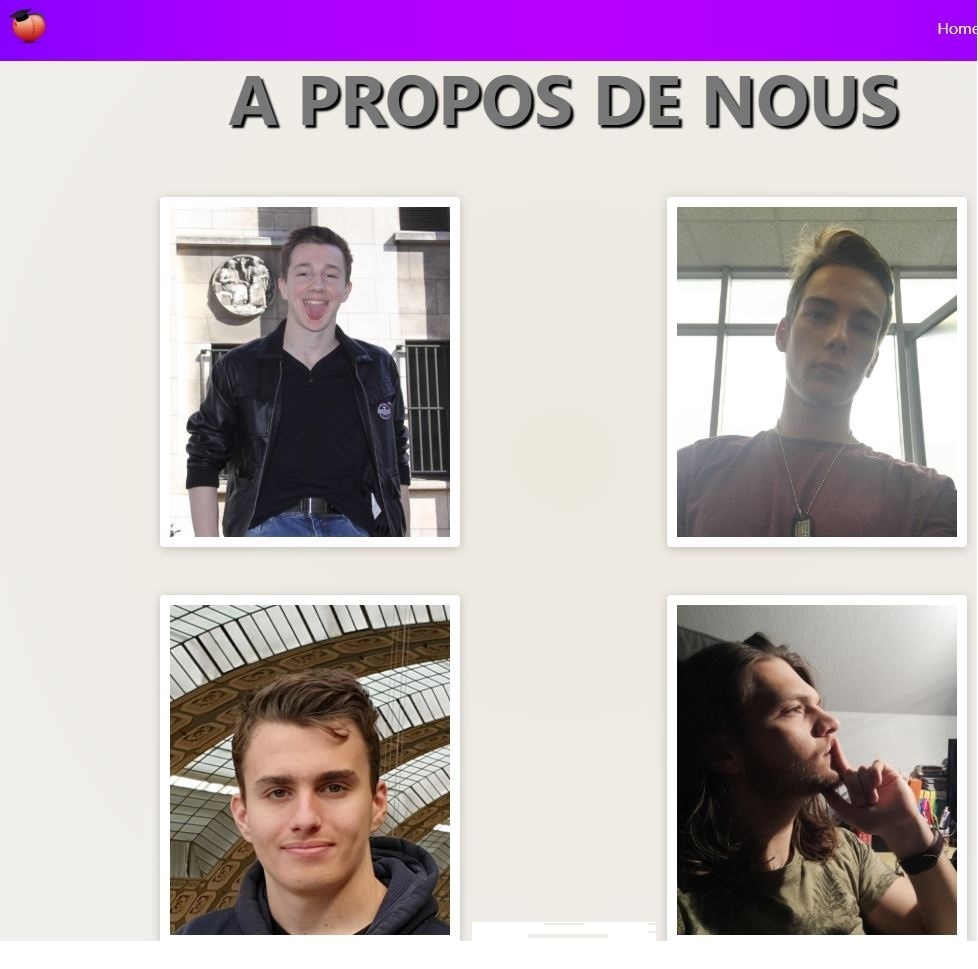
\includegraphics[scale=0.7]{Aboutus.jpg}
	\end{center}
		\caption{Capture d'écran de notre page About (Pensez à passer votre souris sur nos tête)}
\end{figure}
\clearpage
\subsection{Module Administrateur}
Pour un profil classique, les modules de gestion administrateur sont invisibles, à moins qu'un administrateur donne ce grade au profil.\\
En effet pour différencier un profil administrateur d'un autre nous avons créer dans la base de données, plus particulièrement dans la table "user" un paramètre "grade" qui prend soit nouveau si le profil est classique, soit administrateur.\\
\begin{figure}[h!]
	\begin{center}
		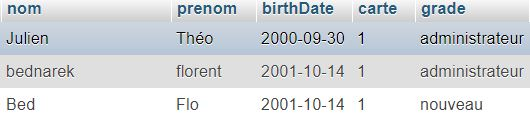
\includegraphics[scale=1.2]{fragBDD.jpg}
	\end{center}
		\caption{Capture d'écran d'un fragment de notre table user}
\end{figure}\\
Cette petite simple variable change grandement les droits et pouvoirs d'un profil sur notre site, en effet en possédant le grade administrateur, un nouveau bouton est visible sur la page principal, le "pannel administrateur".
\begin{figure}[h!]
	\begin{center}
		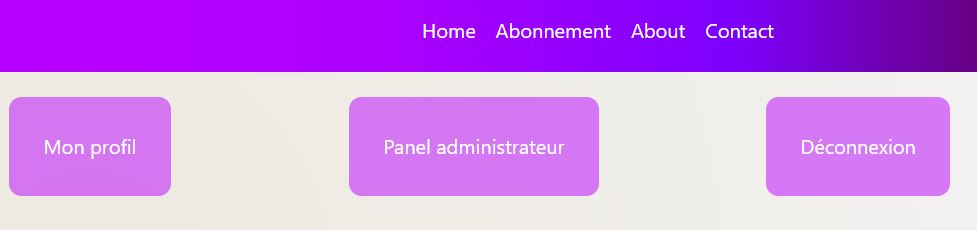
\includegraphics[scale=0.8]{boutonpanel.jpg}
	\end{center}
		\caption{Capture d'écran d'un fragment de notre table user}
\end{figure}
\clearpage
En cliquant sur ce bouton on arrive sur une première page, qui permet la gestion de certification des profils. Quand un utilisateur, s'inscrit et rentre sa carte étudiante, elle doit être vérifié manuellement par un administrateur avant de certifier le profil. Cela permet de donner un vrai sens à la certification sur notre site.\\
\begin{figure}[h!]
	\begin{center}
		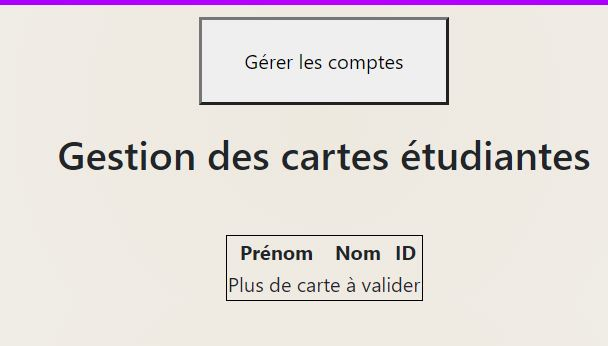
\includegraphics[scale=0.7]{gestioncarte.jpg}
	\end{center}
		\caption{Capture d'écran du panel administrateur }
\end{figure}\\
On y trouve aussi un bouton "Gérer les comptes", en cliquant sur ce bouton on y trouve la liste complète de tous les inscrits, en cliquant sur l Id du profil, l'administrateur peut voir toute les informations stocké dans la table "user". Il peut aussi promouvoir le grade du compte, réinitialiser les likes quotidien, en effet chaque jour un profil normal à 10 likes, mais un administrateur peut réinitialiser ce compteur manuellement. Il peut aussi certifier un profil manuellement sans passer par la gestion de certification vu précédemment, par exemple pour un étudiant en année sabbatique imaginons. Enfin évidemment il peut supprimer le profil d'utilisateur, si celui-ci est Fake, malveillant.
\begin{figure}[h!]
	\begin{center}
		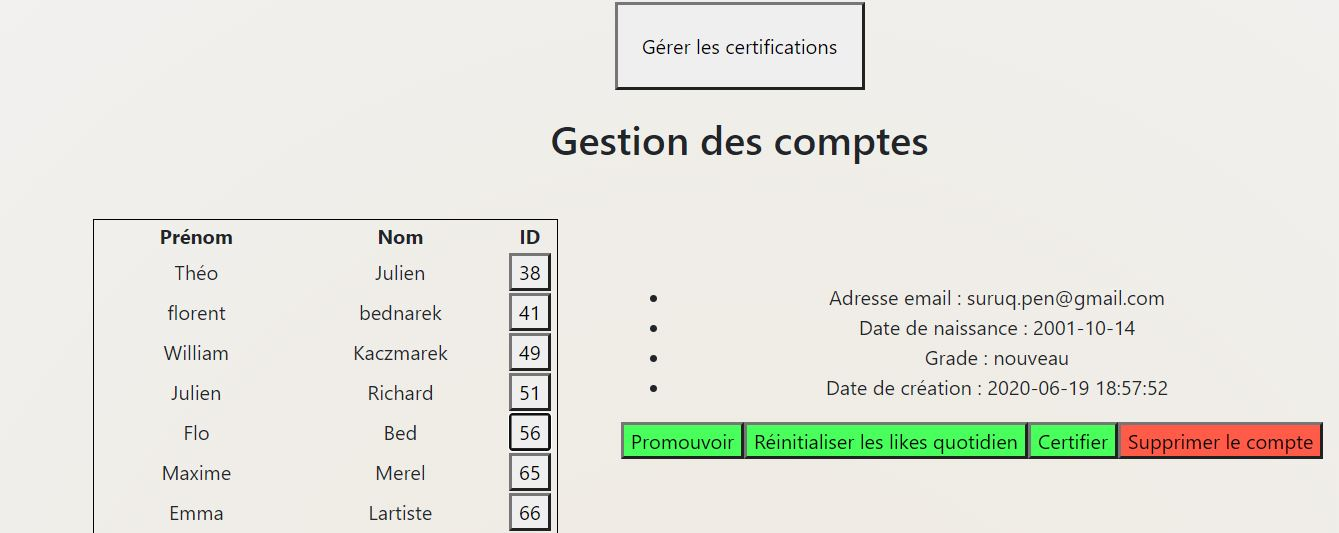
\includegraphics[scale=0.6]{gestioncompte.jpg}
	\end{center}
		\caption{Capture d'écran du panel administrateur après avoir clique sur gestion de compte}
\end{figure}\\
\clearpage
\subsection{Base de données}
	Comme souvent mentionner au dessus, notre site stock les données utilisateurs dans une table nommé "user" mais ce n'est pas la seul table. Nous avons : \\
\begin{itemize}
	\item La table user : Qui stock le nom, prénom, date de naissance, l Id du profil, les Id des profils liké, de même pour les dislikes, son grade, la date de création du compte, son mail, son nombre de like, la date à laquelle se termine son abonnement s'il en possède un et enfin évidemment le mot de passe du compte qui a été haché.
	\item la table préférence : qui stock toutes les préférences d'un profil. Elle est composée de l'Id du profil et ensuite de chaque option possible cheveux, yeux, tranche d'âges etc
	\item la table listeMatch : qui stock les Id des profils qui on matché ensemble, par exemple on peut voir ci-dessous que le profil 38 et 41 on matché.
	\item Toute les autres tables dont le nom est d"id"\_"id", est la discussion entre les profils qui on match, ci-dessous la table "d38\_41" est la discussion entre le match 38 et 41. 
\end{itemize}
\begin{figure}[h!]
	\begin{center}
		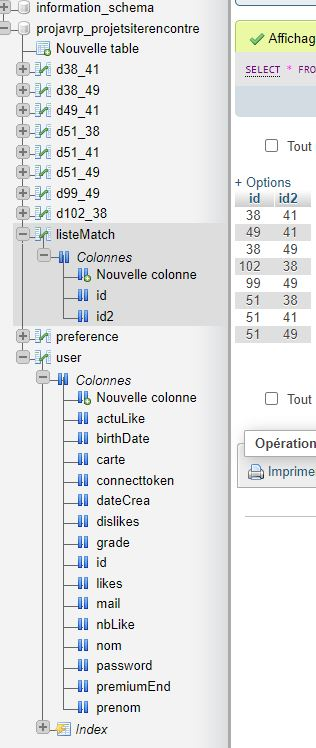
\includegraphics[scale=0.9]{bdd.jpg}
	\end{center}
		\caption{Capture d'écran des tables de notre BDD}
\end{figure}
\clearpage
\section{Réalisation de ce projet et notre organisation}
	Nous avions tous les mêmes compétences en HTML, CSS, Javascript et BDD au début de ce projet grâce au différents TP réalisés pendant le confinement. Toutefois Florent à durant la réalisation de son porte-folio a entendu parlé, de React. React\cite{React} est une librairie/Framework en JavaScript qui permet de créer des interfaces utilisateurs interactives. On peut aussi créer des composants autonomes qui maintiennent leur propre état, puis les assembler pour créer des interfaces utilisateurs complexes. La modernité et les nouvelles possibilités que propose React nous on beaucoup attiré. Nous avons donc décidé de travailler ce projet en React, mais nous ne connaissions rien de cette librairie qui est certes puissante mais possède ses propres règles syntaxique, sa propre structure. Ce fut étrange de devoir réapprendre le développement web d'une certaine manière. Après quelques semaines à ce familiariser avec l'environnement notre groupe était parti est tout c'est bien passé, on pas pu exploiter les fonctionnalités de React comme nous le souhaitions. \\
	Pour bien s'organiser durant les conditions un peu particulière du COVID, nous avons mis en place un GIT pour pouvoir chacun travailler de son coter facilement et qu'on puisse regrouper notre travail facilement sans conflit.
	Pour la répartition du travail on a chacun travailler de notre côté et chacun donnait son avis/ses conseils sur le travails d autrui. L'avantage d'avoir utilisé React, c'est que chacun pouvait développer sur ses composant, et une fois fini ensemble nous construisons notre site avec les composant de chacun.
\section{Déploiement de notre projet}
Pour héberger le Site nous avons utilisé le service GitHub\cite{GitHub} Pages qui est gratuit et propose aucune limite de bande passante, en effet des sites comme twitter utilisent ce service.
cependant nous  ne pouvons pas héberger de bases de donnée sur GitHub et avons donc choisi Planet Hoster\cite{Planet} pour la base de donnée et l'API en php. séparer le front-end et la back-end nous a permis de réduire la demande sur un seul hébergeur et ainsi rend donc le site plus fluide.\\
Voici le lien de notre site hébergé en ligne :
\href{https://florentbednarek.github.io/projetwebEISTI}{\textbf{\emph{Notre Site}}}

\section{Conclusion de ce projet}

			\begin{thebibliography}{10}
			\bibitem{React}
			Site officiel de React
			\emph{\href{https://fr.reactjs.org/}{https://fr.reactjs.org/}}
			\bibitem{GitHub}
			GitHub Page hébergement de notre site
			\emph{\href{https://pages.github.com/}{https://pages.github.com/}} 
			\bibitem{Planet}
			Planet Hoster hébergement de notre BDD
			\emph{\href{https://www.planethoster.com/fr/}{https://www.planethoster.com/fr/}}
		\end{thebibliography}
\end{document}
